% !TeX root = ../tfg.tex
% !TeX encoding = utf8

\chapter{Introduction to Quantum Computing} \label{ch:2-IntroQC}



In 1981 at MIT, the first Physics of Computation Conference was held, organized by MIT and IBM, which brought together 50 scientists for three days. It was the founding forum to discuss the possibility of taking signals from the natural world to address the problems of designing increasingly powerful and efficient forms of computation. Attendees debated the limitations and possibilities brought about by the shrinking of computer components (Moore's Law). Ultimately, it was the time and place to discuss the intersection of the physical sciences and computer sciences, which helped to connect the paths of both disciplines. Today, this conference holds more weight than they could have imagined at the time. Perhaps due to the significance of its sponsoring institutions and the fame of some attendees, such as Freeman Dyson, John Wheeler, and Richard Feynman, we can say that it was the birthplace of physics of computation and especially the now flourishing field of quantum computing.

The opening speech of the Physics of Computation Conference was delivered by Richard Feynman and was titled ``Simulating physics with computers''. As the title suggests, it explores the idea of how physics can be simulated using computers, which is related to the possibilities of computers and also the possibilities of physics. Throughout the speech, he poses a series of questions.

First, he addresses the question: What type of physics will be simulated with computers? Classical physics is often described using differential equations, but the physical world is quantum, so the problem he raises is simulating quantum physics.

\begin{quote}
    ``And I'm not happy with 
all the analyses that go with just the classical theory, because nature isn't 
classical, dammit, and if you want to make a simulation of nature, you'd 
better make it quantum mechanical, and by golly it's a wonderful problem, 
because it doesn't look so easy."
\end{quote}

The idea that Richard Feynman explores is whether there is an exact simulation in which the computer will do exactly the same as nature.

So, how can quantum mechanics be simulated? To answer this question, Richard Feynman concludes that the only possibilities are: to use a probabilistic computer or to do it with a new type of computer, a quantum computer built with elements of quantum mechanics that obey the laws of quantum mechanics. He asserts that a quantum system can be simulated with quantum computational elements. He is not referring to a Turing machine but to a machine of a different type. Feynman believes that it is true that with an appropriate class of quantum machines, one could simulate any quantum system, including the physical world.

In his speech, Feynman only outlines ideas about what this quantum computer would be like. He also raises the question of which types of quantum systems are equivalent and the possibility of finding a class that could simulate all quantum systems. This leads to the question of whether a universal quantum computer could be found. He suggests using linear operators in a two-state quantum system as the basis for simulating any quantum system.

In the final part of the conference, he argues whether a quantum system can be probabilistically simulated with a classical universal probabilistic computer, meaning a computer that would obtain the same probabilities as the quantum system. He concludes that this is definitely not the case and that it is impossible to represent the results of quantum mechanics with a classical universal device.

Feynman proposes this union between computing and physics because he claims that the discovery of computing has proven very useful in many branches of human reasoning. For example, attempting to create a computer that understands our language made us realize how poor our understanding of language and grammar theory was. Similarly, we have gained some insights about psychology and philosophical issues by approaching them from a computational perspective. Feynman's intention was that introducing computational approach would provide us with new ideas if they were necessary.

\section{Review on Hilbert spaces}
Quantum theory can me understood as an extension of classical probability theory to make predictions about the stochastic outcomes of measurements on microscopic objects (such as electrons, protons, atoms, etc.) that form quantum systems.

The rigorous formulation of this requires some mathematical tools and notions that we will review next.

\begin{definicion}[Inner product]
    Let X be a vector space, that is, 
    \begin{equation*}
        \psi,\phi \in X \text{ and } a,b \in \mathbb{C} \text{ verify } a\psi+b\phi \in X
    \end{equation*}
    The scalar product or inner product in $X$ is an application 
    \begin{align*}
        \braket{\cdot,\cdot}:X\times X &\longrightarrow \mathbb{C} \\
        (\psi, \phi) &\longmapsto \braket{\psi,\phi}
    \end{align*}
    That verifies for all $\phi, \psi, \phi_1, \phi_2 \in X$ y $a,b\in \mathbb{C}$
        \begin{enumerate}
            \item It is hermitian: $\braket{\psi,\phi} = \overline{\braket{\psi,\phi}}$ 
            \item It is positive definite: $\braket{\psi,\psi}\geq 0$ y $\braket{\psi,\psi}=0 \Leftrightarrow \psi = 0$
            \item It is sesquilinear, that is
                \begin{itemize}
                    \item $\braket{\psi,a\phi_1+b\phi_2}=a\braket{\psi,\phi_1}+b\braket{\psi,\phi_2}$ (Linearity of the second entry)
                    \item $\braket{a\psi_1 + b\psi_2,\phi}=\overline{a}\braket{\psi_1,\phi}+\overline{b}\braket{\psi_2,\phi}$ (Antilinearity of the first entry)
                \end{itemize}
        \end{enumerate}
\end{definicion}

\begin{definicion}[Pre-Hilbert space]
    If $\braket{\cdot , \cdot}$ is a inner product in a vector space $\mathbb{H}$, we will say that $\mathbb{H}$ is a pre-Hilbert space.
\end{definicion}

This inner product induces a norm in $\mathbb{H}$, 
\begin{align}
    || \cdot ||:\mathbb{H} &\longrightarrow \mathbb{R}\\
    \psi &\longmapsto \sqrt{\braket{\psi,\psi}}
\end{align}

\begin{definicion}
    A normed space $M$ is complete if every Cauchy sequence in $M$ is convergent. That is, if $\left\lbrace x_n\right\rbrace_{n \in \mathbb{N}}$ is a sequence in $M$ such $\forall \epsilon >0\,\,\exists n_0 \in \mathbb{N}$ that $n,m \geq n_0$, $||x_n - x_m|| < \epsilon$, then $\left\lbrace x_n \right\rbrace$ converges in $M$. 
    This spaces receive the name of \textbf{Banach spaces}. 
\end{definicion}

\begin{definicion} [Hilbert space]
    A Hilbert space $\mathbb{H}$ is a pre-Hilbert space that is complete respect to the norm induced by the inner product.
\end{definicion}

Equivalently, a Hilbert space is a Banach space with the norm induced by the inner product. 

\begin{definicion}[Separable space]
    A metric space $M$ is separable if there exists a subset $N \subset M$ that is countable and dense.
\end{definicion}

Now we will quickly revise the basic concepts of linearly independence, span and basis.
\begin{definicion}
    Let $X$ be a pre-Hilbert space and $J$ an index set.
    
    A set of vectors $\left\lbrace v_i \, | \, i \in J\right \rbrace \subset X$ is \textbf{linearly independent} if the coefficients $\alpha_i \in \mathbb{C},\, i \in J$ such that
    $$\sum_{i \in J}\alpha_i v_i = 0$$
    only holds if $a_i=0$ for all $i\in J$.
    
    A set of vectors $\left\lbrace v_i \, | \, i \in J\right \rbrace \subset X$ \textbf{spans} X if for every $\omega \in X$, there are coefficients $\alpha_i \in \mathbb{C}$ , $ i\in J$ such that
    $$\omega =\sum_{I \in J} \alpha_i v_i$$ Therefore, we denote it as $$X = \mathrm{span}\left\lbrace v_i \, | \, i \in J\right \rbrace$$

    A linearly independent set $\left\lbrace v_i \, | \, i \in J\right \rbrace$ that spans $X$ is called a \textbf{basis} of $X$. 

    An \textbf{orthonormal basis} $\left\lbrace e_i \,\, | \, i \in J\right \rbrace $ is a basis whose vectors are unitary ($||e_i||=1\, \forall i \in J$) and verify
    $$\braket{e_i|e_j}=\delta_{i,j}=
    \left\{ \begin{array}{lcc} 
    0 & \mathrm{if} & i \neq j \\
    1 & \mathrm{if} & i = j 
    \end{array} \right.$$
\end{definicion}

\begin{teorema}
    Every separable Hilbert space has an orthonormal basis.
\end{teorema}
\begin{proof}
    Let $\mathbb{H}$ be a Hilbert space and $\left\lbrace u_n \right\rbrace$ be a countable dense subset of $\mathbb{H}$. We consider the nondecreasing sequence of linear spaces $\left\lbrace E_i \right\rbrace = \textbf{span}\left\lbrace u_1, u_2, ..., u_i\right\rbrace$ such that $ \bigcup_{i=1}^{\infty} E_i$ is dense in $\mathbb{H}$. 

    Let's pick any unit vector $u_1$ in $E_1$. If $E_2 \neq E_1$, there is some vector $u_2 \in E_2$ such that $\left\lbrace u_1, u_2 \right\rbrace$ is an orthonormal basis of $E_2$. By repeating this iterative construction, we obtain an orthonormal basis of $\mathbb{H}$. \cite{brezis2011functional}
\end{proof}

Now we will get introduced to the notion of linear functional.

\begin{definicion}[Linear operator]
    Let $X$ and $Y$ be to vector spaces. A linear operator from $X$ to $Y$ is an application $T: X \longrightarrow Y$ that verifies
    $$T(\lambda_1 x_1 + \lambda_2 x_2) = \lambda_1 T(x_1) + \lambda_2 T(x_2) \quad \forall \lambda_1, \lambda_2 \in \mathbb{K},\,x_1, x_2 \in X$$

    If $Y = \mathbb{K}$ the linear operator $T$ receives the name of \textbf{linear functional}.
\end{definicion}

\begin{proposicion}[Continuous operator]
    Let $X$ and $Y$ be normed vector spaces and $T: X \longrightarrow Y$  a linear operator. Then $T$ is continuous if and only if $\exists M \in \mathbb{R}_0^{+}$  such that $$||T(x)|| \leq M ||x|| \quad \forall x \in X$$
\end{proposicion}

\begin{definicion} [Operator space]
    Given $X$ and $Y$ normed vector spaces over $\mathbb{K}$, we denote $\mathcal{L}(X,Y)$ the set of all linear operators from $X$ to $Y$. Provided with the operations:
    \begin{itemize}
        \item $\forall T,S \in \mathcal{L}(X,Y), \, (T+S)(x) = T(x) + S(x) \quad \forall x \in X$
        \item $\forall \lambda \in \mathbb{K},\,\forall T \in \mathcal{L}(X,Y), \, (\lambda T)(x) = \lambda T(x) \quad \forall x \in X$
    \end{itemize}
    The set $\mathcal{L}(X,Y)$ has structure of vector space. 
\end{definicion}

\begin{definicion}[Dual space]
    Let $X$ be a normed vector space over $\mathbb{K}$. The operator space from $X$ to $\mathbb{K}$, $\mathcal{L}(X,\mathbb{K})$ of all linear and continuous functionals in $X$ is called dual space and it is denoted as $X^{*}$. It is provided with the norm
    
    $$||f||_{X^{*}} = \min \left \lbrace M \in \mathbb{R}_0^{+} :\, |f(x)| \leq M||x||_{X} \quad \forall x \in X \right\rbrace$$
\end{definicion}


In a Hilbert space, we can define linear functionals $T_{\psi}$ for every $\psi \in \mathbb{H}$ with the help of the scalar product:
\begin{align}
    T_{\psi}: &\mathbb{H} \longrightarrow \mathbb{C} \\
    &\varphi \longmapsto \braket{\psi, \varphi}
\end{align}

By virtue of the Theorem of Riesz,  \autoref{th:Riesz theorem}, for each functional $T \in \mathbb{H}^{*}$, there exists a unique $\psi \in X$ such that $T(x)=\braket{x,\psi}\quad \forall x \in X$. 

This means that there is a bijection between $\mathbb{H}$ and its dual space $\mathbb{H}^{*}$: every linear and continuous functional from $\mathbb{H}$ to $\mathbb{C}$ is uniquely represented as a scalar product with a suitable vector in $\mathbb{H}$.

Therefore, $\mathbb{H}$ and $\mathbb{H}^{*}$ are isomorphic, in particular, if $\mathbb{H}$ is a separable Hilbert space, the dual space $\mathbb{H}^{*}$ is a vector space with the same dimension as $\mathbb{H}$.

This fact suggests the \textbf{Bra-ket notation} introduced by Paul Dirac, extensively used in Quantum Mechanics.
\begin{itemize}
    \item Ket-vectors are elements of $\mathbb{H}$. A vector $\varphi \in \mathbb{H}$ in the Hilbert space is denoted in Dirac's notation as the ket $\ket{\varphi} \in \mathbb{H}$.

    \item Bra-vectors are elements of the dual space $\mathbb{H}^{*}$. A functional $T_{\phi} \in \mathbb{H}^{*}$ is denoted in Dirac's notation as the bra $\bra{\phi} \in \mathbb{H}^{*}$.

    \item The action of a functional $\bra{\phi} \in \mathbb{H}^{*}$ on a vector $\ket{\varphi} \in \mathbb{H}$ is denoted as the braket $\braket{\phi | \varphi} = \braket{\phi, \varphi} \in \mathbb{C}$. Note the scalar product.
\end{itemize}

In other words, every ket $\ket{\varphi}$ has a corresponding $\bra{\varphi}$ that is unique. The scalar product of two vectors (kets) $\ket{\phi}$ and $\ket{\varphi}$ is given by the braket $\braket{\phi | \varphi}= \braket{\phi , \varphi}^{*}$

A basis of the Hilbert space $\mathbb{H}$ can be denoted according to Dirac's notation as $\left\lbrace \ket{\phi_i} \, | \, i \in J \right\rbrace$ and we can express any ket $\ket{\varphi} \in \mathbb{H}$ as 
$$\ket{\varphi} = \sum_{i \in J}\ket{\phi_i} \alpha_i$$
where $\alpha_i$ are the components of $\ket{\varphi }$ in the basis $\left\lbrace \ket{\phi_i} \, | \, i \in J \right\rbrace$.

Now, let $\left\lbrace \ket{e_i} \, | \, i \in J \right\rbrace$ be an orthonormal basis of $\mathbb{H}$. The coefficients of any vector can be obtained from the inner product, since $\ket{\varphi} = \sum_{i \in J}\ket{e_i} \alpha_i $, then
$$\braket{e_k|\varphi}= \sum_{i \in J}\braket{e_k|e_i} \alpha_i = \sum_{i \in J} \delta_{ki}\alpha_i = \alpha_k$$

As a result,
$$\ket{\varphi} = \sum_{i \in J}\ket{e_i} \braket{e_i|\varphi}$$

Regarding the inner product of two vectors, we can use its representation in an orthonormal basis as
\begin{align}
    \ket{\varphi} &= \sum_{i \in J}\ket{e_i} \varphi_i = \sum_{i \in J}\ket{e_i} \braket{e_i|\varphi} \\
    \ket{\phi} &= \sum_{i \in J}\ket{e_i} \phi_i = \sum_{i \in J}\ket{e_i} \braket{e_i|\phi}
\end{align}
$$\braket{\phi | \varphi} = \sum_{i \in J}\braket{\varphi | e_i} \braket{e_i|\phi} = \sum_{i \in J}\braket{e_i | \varphi}^{*} \braket{e_i|\phi} = \sum_{i \in J}\varphi_i^{*} \phi_i = \braket{\varphi, \phi}^{*} $$

Indeed, the isomorphism between $\mathbb{H}$ and $\mathbb{H}^{*}$ is given by the adjoint relation:
\begin{align}
    \mathbb{H} &\longrightarrow \mathbb{H}^{*} \\
    \ket{\varphi} &\longmapsto \bra{\varphi} = \ket{\varphi}^\dag =\sum_{i \in J} \varphi_i^{*} \bra{e_i}
\end{align}
Thus, there is an adjoint basis in $\mathbb{H}^{*}$
$$\left\lbrace \ket{e_i}\right\rbrace  \longmapsto \left\lbrace \bra{e_i}\right\rbrace$$

\begin{definicion}[Adjoint operator]
    Let $X$ and $Y$ be normed spaces. Consider the linear operator $T$ from $X$ to $Y$. The adjoint operator of $T$, noted as $T^\dag$ is the operator $T^\dag : Y^* \longrightarrow X^* $ defined as $\forall g \in Y^*,\, T^\dag (g)$ is the functional given by $(T^\dag g)(x) = g(T(x)) \quad \forall x \in X$. 
    When $X$ and $Y$ are finite spaces of dimension $n$, then $T \in \mathcal{M}_{n \times n}$. Thus, its adjoint $T^\dag$ is given by $(T^\dag)_{ij}= T^*_{ji}$. 
\end{definicion}

When $T$ is a linear operator in a Hilbert space $\mathbb{H}$, we can apply the Riesz theorem, \autoref{th:Riesz theorem}, on both sides of the definition $(T^\dag g)(x) = g(T(x))$ to obtain that the adjoint operator realices the following equivalent identity: $\braket{T^\dag (u) , v} = \braket{u, T(v)}, \, \forall v \in \mathbb{H}$.


\begin{definicion}[Self-adjoint operator]
    A linear operator $T$ in a Hilbert space $\mathbb{H}$ is a self adjoint operator, also known as Hermitian operator, if its adjoint is itself: $T^\dag =T$. This is equivalent to say $\braket{T(x), y} = \braket{x, T(y)} \quad \forall x, y \in \mathbb{H}$.
\end{definicion}

\begin{definicion}[Unitary operator]
    An operator $T$ is unitary if $T^\dag T = T T^\dag = \mathbb{1}$
\end{definicion}

\begin{definicion} [Outer product]
    Let $X$ and $Y$ be vector spaces. The outer product of $v \in X$ and $w \in Y$, using Dirac's notation is $$\ket{w} \bra{v}$$ is the only linear operator such that 
    $$(\ket{w} \bra{v}) \ket{x} = \braket{v,x} \ket{w} \quad \forall \ket{x} \in X$$.
\end{definicion}

Lastly, we will remember the concepts of eigenvalues and eigenvectors.

\begin{definicion}[Eigenvalue and eigenvector]
    Given $X$ a vector space over $\mathbb{K}$, $T \in \mathcal{L}(X)$ and $v \in X$. If there exist a $\lambda \in \mathbb{K}$ such that
    \begin{equation}
        T v = \lambda v
    \end{equation}

    Then, $\lambda$ is an eigenvalue of $T$ and $v$ is a eigenvector of $T$. 
\end{definicion}

Next, we will present two definitions that allow us to quantify the characteristics of a system defined within a Hilbert space.

\begin{definicion}[Observable]
    In physics, an observable, such as position or momentum, are physical quantities governed by a real-valued function in the case of classical mechanics. In the case of quantum mechanics, an observable is given by an operator that can be measured. 
\end{definicion}

\begin{definicion}[Expected value]
    Given an operator $T$, the expected value $\braket{T}$ is defined as the probabilistic value expected to be obtained when a measurement of the observable associated with $T$ is performed. If the system is in a state $\psi$, the expected value of $T$ is given by $\braket{T}_{\psi}=\braket{\psi | T | \psi}$.     
\end{definicion}

Finally, we will point out a particular type of observable:

\begin{definicion}[Hamiltonian]
    In quantum mechanics, the operator corresponding to the total energy (kinetic and potential) of the system is called the Hamiltonian.
\end{definicion}


\section{Postulates of Quantum Mechanics} \label{sec: postulates of QM}
Now, we will formulate the framework of quantum mechanics for finite-dimensional systems with the guidance of a number of postulates which specify the mathematical objects used to describe certain physical entities. We will follow \cite{nielsen_chuang_2010}.

\subsection{State space} \label{sec: state space}
\begin{tcolorbox}[title=Postulate $1$]

    Associated to any isolated physical system is a complex vector space with inner product (that is, a Hilbert space) known as the \textbf{state space} of the system. The system is completely described by its \textbf{state vector}, which is a unit vector in the system's state space.
\end{tcolorbox}

A quantum system with a state vector $\ket{\psi}$ is called a pure state. However, usually systems cannot be described by an unique pure state, instead they are in a statistical ensemble of different pure states, each of them with its own probability. In this case, the state of a system is given by a operator called \textbf{density operator} or \textbf{density matrix}, defined by
\begin{equation}
    \rho = \sum_{i=1}^{n} p_i \ket{\psi_i}\bra{\psi_i}
\end{equation}
where all $p_i \geq 0 $ and $\sum_i p_i = 1$.

Additionally, a density matrix has the following properties:
\begin{enumerate}
    \item $\rho$ is self-adjoint $$\rho^{\dag}=\rho$$
    \item $\rho$ has trace $1$ $$\mathrm{Tr}(\rho) = 1$$
    \item $\rho$ is positive $$\rho \geq 0$$
    
\end{enumerate}


This postulate does not provide the state space for a given system. Although, for the purpose of computation, the state spaces to consider should be discrete and finite-dimensional Hilbert spaces. These are isomorphic to the $\mathbb{C}^K$, and a quantum state therefore has a representation as a complex-valued vector.

The simplest quantum mechanical system is the one qubit system.

\begin{definicion}[Qubit]
    A state vector of the state space $\mathbb{C}^2$ is called a qubit.
\end{definicion}

Now we pick up again Dirac's notation and we assume $\ket{0}$ and $\ket{1}$ form an orthonormal basis in a 2-dimensional Hilbert space. Thus, any state vector in the state space can be written as a linear combination of the basis vectors:
$$\ket{\varphi} = \alpha \ket{0} + \beta \ket{1}$$

where $\alpha, \beta \in \mathbb{C} $ are called amplitudes. A state vector is by definition unitary. This condition translates into $\braket{\varphi | \varphi} = 1$, which is equivalent to $|a|^2 + |b|^2 = 1$. This is known as normalization condition. 

A qubit is the minimal information unit in quantum computing. It is the analogous to the classical bit in classical computation. Intuitively, the states $\ket{0}$ and $\ket{1}$ are equivalent to the values 0 and 1 which a bit may take. The difference relies on the fact that $\ket{0}$ and $\ket{1}$ are not the only states of a qubit, one can prepare a qubit in any arbitrary superposition of these two states: $\alpha \ket{0} + \beta \ket{1}$. 

As we know, classical computation is built based on bits. Similarly, quantum computing is constructed upon the qubit. 

We conclude with some usual terminology. The orthonormal basis of the state space receives the name of computational basis. In the case of the state space of a 1-qubit system, the constituents of the computational basis are the column vectors
\begin{equation}
    \ket{0} =
    \begin{bmatrix}
    1\\
    0\\
    \end{bmatrix}
    \quad \quad
    \ket{1} =
    \begin{bmatrix}
    0\\
    1\\
    \end{bmatrix}  
\end{equation}

and hence,
\begin{equation}
    \ket{\varphi}= \alpha \ket{0} + \beta \ket{1} = \alpha \begin{bmatrix}
    1\\
    0\\
    \end{bmatrix} + \beta \begin{bmatrix}
    0\\
    1\\
    \end{bmatrix} = \begin{bmatrix}
    \alpha\\
    \beta\\
    \end{bmatrix} 
\end{equation}

Additionally, taking into account a general orthonormal basis $\ket{e_i}$ of $\mathbb{H}$, with $\braket{e_i| e_j} = \delta_{ij}$, we realise that any $\ket{\varphi} \in \mathbb{H}$
$$\ket{\varphi} = \sum_i \braket{e_i|\varphi} \ket{e_i}$$

This previous equation also implies the \textbf{completeness relation}: $$\sum_i \ket{e_i}\bra{e_i} = \mathbb{1}$$ which holds for any orthonormal basis $\ket{e_i}$ of a finite $\mathbb{H}$.

We can generalise this to the case of $n$-qubits, thus we say that any linear combination $\sum_{i} \alpha_i \ket{\phi_i}$ is a superposition of the states $\ket{\phi_i}$ with amplitude $\alpha_i$ for the state $\ket{\phi_i}$.

In particular, we will see that the state space will be $\mathbb{C}^{2^n}$ for an $n$-qubit quantum computation system.

In conclusion, this first postulate sets the framework in which quantum mechanics takes place: Hilbert spaces. In particular, for quantum computation where we work with a finite number of qubits, we will consider finite Hilbert spaces. Linear algebra and functional analysis provide us the tools we need to operate in them. It is worth pointing out that the definition of a qubit is derived from quantum physics and mathematics, describing the qubit as a mathematical object independent of its physical implementation. This enables the construction of quantum computing regardless of its physical implementation.

\subsection{Observables} \label{sec: observables}
\begin{tcolorbox}[title=Postulate $2$]

    An observable, that is, a physically measurable quantity of a quantum system is represented by a Hermitian or self-adjoint operator on a Hilbert space $\mathbb{H}$.
\end{tcolorbox}

Let $\mathcal{M}$ be a self-adjoint operator in $\mathbb{H}$ that acts on ket $\ket{\varphi}$ characterising the system. By virtue of the spectral theorem, \autoref{th:spectral theorem}, such self-adjoint operators have a diagonal matrix representation in terms of the orthonormal basis of eigenvectors
 $\left\lbrace \ket{\mu_j} \right\rbrace$, with the eigenvalues in the diagonal.
We can formulate this like
\begin{equation}
    \mathcal{M}=\sum_{k} \lambda_k \ket{\lambda_k} \bra{\lambda_k}
\end{equation}
where $\lambda_k$ are the eigenvalues and $\ket{\lambda_k}$ their corresponding eigenvectors. 

The only possible values that the observable can take are its eigenvalues, which are real because the observable is a self-adjoint operator. Therefore, the values of physical observables are always real numbers.

\subsection{Time Evolution}\label{sec: time evolution}

\begin{tcolorbox}[title=Postulate $3$]

    The evolution of a closed quantum system is described by a unitary transformation. That is, the state $\ket{\varphi}$ of the system at time $t_1$ is related to the state $\ket{\varphi^\prime}$ of the system at time $t_2$ by a unitary operator $U$ which depends only on the times $t_1$ and $t_2$. 
    \begin{equation}
        \ket{\varphi^\prime} = U(t_1,t_2) \ket{\varphi}
    \end{equation}
\end{tcolorbox}

This postulate encloses how a quantum state $\ket{\varphi}$ evolves through time but it does not tell you which unitary operators describe this evolution. In the context of quantum computing, any unitary operator can be realized in realistic systems and we will define them. While we may not know the specific unitary transformation for an arbitrary system, we are able to create systems that follow specific desired transformations. These principles form the foundation of quantum gates and quantum circuits

Now we will have a look at an example of an unitary operator on a single qubit which is important in quantum computation. We will detail at the end of this chapter a collection with the most important quantum gates.

\begin{ejemplo}[NOT gate]
    Let's consider the operator given by the matrix 
    \begin{equation}
        X = \begin{bmatrix}
        0&1\\
        1&0\\
        \end{bmatrix} 
    \end{equation}
    known as the Pauli X matrix $\sigma_x$ or NOT gate. It is evidently a unitary operator, since $X^\dag X = \mathbb{1}$. 

    We can observe that 
    \begin{equation}
        X \ket{0}= \begin{bmatrix}
        0&1\\
        1&0\\
        \end{bmatrix} 
        \begin{bmatrix}
        1\\
        0\\
        \end{bmatrix} =
        \begin{bmatrix}
        0\\
        1\\
        \end{bmatrix} = \ket{1}
    \end{equation}
    which is precisely what Postulate 3 states,  the evolution
    of our state vector following the unitary operator $X$: $X \ket{0} = \ket{1}$. 
\end{ejemplo}

It is worth pointing out two aspects of this postulate.
\begin{itemize}
    \item It requires that the physical system system is closed, that is, it is not interacting in any way with the exterior. This is quite a strict assumption, since in reality, all systems interact at least somewhat with others and the only real closed system is the universe as a whole. However, some systems can be described to a good approximation as being closed.

    \item It refers to the description of evolution of a closed quantum system at two different times $t_1$ and $t_2$. It is natural to consider the evolution of a quantum system in continuous time. For this, we will consider the Schrödinger equation, which provides a continuous time description of a closed system. We can redefine the Postulate 3 in these terms.
\end{itemize}

\begin{tcolorbox}[title=Postulate $3^\prime$]

    The time evolution of the state of a closed quantum system is described by the Schrödinger equation,
    \begin{equation}
        i \hbar \frac{d \ket{\phi}}{dt} = H \ket{\phi}
    \end{equation}
    where $\hbar$ is a physical constant known as Plank's constant and $H$ is a fixed Hermitian operator known as the Hamiltonian of the closed system.
\end{tcolorbox}

The Hamiltonian of the system is fixed and it represents the energy of the system. The value $\hbar$ is physical constant that we can absorb into the Hamiltonian to simplify the equation. At the end of the day, a Hamiltonian is an observable and we can apply the results from Postulate 2. As we will see later, circuits in quantum computers are built up from elementary gates that act as unitary operators on the states. In order to implement such gates, one then tries to create Hamilton operators that generate a time evolution implementing the desired gate.


Since the Hamiltonian is a self-adjoint operator, by the Spectral decomposition theorem, \autoref{th:spectral theorem}
$$H = \sum_{j} \lambda_j \ket{\lambda_j} \bra{\lambda_j}$$
with eigenvalues $\lambda_j$ and corresponding eigenvectors $\ket{\lambda_j}$. Conventionally, $\ket{\lambda_j}$ are referred to as \textit{energy eigenstates} and the eigenvalues $\lambda_j$ as the energy of the state $\ket{\lambda_j}$. 

Now we will consider the example for a single qubit that has Hamiltonian $$H=\hbar \omega X, \quad \omega >0,\, 
        X = \begin{bmatrix}
        0&1\\
        1&0\\
        \end{bmatrix} $$
to check that there is a one to one correspondence between the continuous time-varying postulate $3^\prime$ using the Hamiltonian and the more stationary discrete-time version using the unitary operator (Postulate 3). 

The energy eigenstates of this Hamiltonian are the ones of $X$: \\$(\ket{0} + \ket{1})/\sqrt{2}$ and $(\ket{0} - \ket{1})/\sqrt{2}$ with corresponding energies (eigenvalues): $\hbar \omega$ and $-\hbar \omega$. 

The solution to Schrödinger's equation is
$$\ket{\phi(t_2)} = \exp{\left[ \frac{-i H(t_2-t_1)}{\hbar}\right] } \ket{\phi(t_1)}$$

Now, we define the operator 
$$U(t_1, t_1) = \exp{\left[ \frac{-i H(t_2-t_1)}{\hbar}\right] } \ket{\phi(t_1)}$$
which is an unitary operator. In fact, any unitary operator $U$ can be expressed as $U=\exp (iK)$ for some Hermitian operator K. 

Therefore, we obtain that the state $\ket{\phi(t_2)}$ is related with the state $\ket{\phi(t_1)}$ through the unitary operator $U(t_1, t_2)$:
$$\ket{\phi(t_2)} = U(t_1,t_2) \ket{\phi(t_1)}$$

Like this, we have obtained the equivalence of postulates $3$ and $3^\prime$.

In quantum computing, the circuit model usually consists of ``applying'' a unitary operator to a quantum system. A priori we may think that this act contradicts what we have just stated about the evolution of a closed quantum system because we are interacting with it and thus, the system is not closed. It turns out to be possible to write down a time-varying Hamiltonian for a quantum system that is not closed but overall the system evolves according to Schrödinger's equation with a time-varying Hamiltonian to some good approximation. The main exception to this are measurements, which we will dive into next.

\subsection{Measurements}\label{sec: measurements}
A closed quantum system evolves according to unitary evolutions by virtue of Postulate 3. But the moment there is an observation of the system, this interaction makes the system no longer closed and thus, not necessarily subject to unitary evolution. To explain what happens in this context we will introduce the following postulate, which describes the effects of measurement operations on quantum systems.

\begin{tcolorbox}[title=Postulate $4$]

    Quantum measurements are described by a collection $\left\lbrace M_m \right\rbrace$ of \textit{measurement operators}. These are operators acting on the state space of the system being measured. The index $m$ refers to the measurement outcomes that may occur in the experiment. If the state of the quantum system is $\ket{\phi}$ immediately before the measurement then the probability that result $m $ occurs is given by 
    $$p(m) = \braket{\phi | M_m^{\dag}M_m | \phi }$$
    and the state of the system after the measurement is 
    $$\frac{M_m \ket{\phi}}{\sqrt{\braket{\phi | M_m^{\dag}M_m | \phi }}}$$

    The measurement operators satisfy the \textbf{completeness equation}:
    $$\sum_m M_m^{\dag}M_m = \mathbb{1}$$
    
\end{tcolorbox}

The completeness equation expresses the fact that probabilities of the possible different outcomes sum one. 
    $$\sum_m p(m) = \sum_m \braket{\phi | M_m^{\dag}M_m | \phi } = \braket{\phi |\sum_m M_m^{\dag}M_m | \phi } = \braket{\phi|\phi} = 1$$
Reciprocally, the fact of every state verifying this equation implies the completeness equation.

In the context of quantum computing, an important measurement is the measurement in the computational basis. Now we will review it for the case of a single qubit. 

When measuring a qubit there are two possible outcomes: $\ket{0}$ and $\ket{1}$ defined by two measurement operators $M_0 = \ket{0}\bra{0}$ and $M_1=\ket{1} \bra{1}$ respectively. We can observe that:
\begin{itemize}
    \item These measurement operators are Hermitian: $$M_i^{\dag} = (\ket{i} \bra{i})^{\dag} = (\bra{i})^{\dag} (\ket{i)}^{\dag} = \ket{i} \bra{i} = M_i$$
    \item They verify $M_i^2 = \ket{i} \braket{i|i} \bra{i} = \ket{i} \bra{i} = M_i$
    \item The computational basis is orthonormal and thus, fulfills the completeness relation: 
    $$\sum_i \ket{i} \bra{i} = 1$$
    Then, the completeness equation also holds:
    $$\sum_i M_i^{\dag}M_i = \sum_i M_i^2 = \sum_i M_i = \sum_i \ket{i} \bra{i} = 1$$
\end{itemize}

Now, let's measure. Suppose we have the state $\ket{\phi} = \alpha \ket{0} + \beta \ket{1}$. The probability of obtaining measurement outcome $0$ is 
$$p(0)=\braket{\phi | M_0^{\dag}M_0 | \phi } = \braket{\phi | M_0 | \phi} = |\alpha|^2$$
Analogously, the probability of obtaining the measurement outcome $1$ is $p(1)=|\beta|^2$.

The completeness equation $|\alpha|^2 + |\beta|^2 = 1$ is fulfilled thanks to the state vector normalization condition. 

After measurement, depending on the measurement outcome $0$ or $1$, the state would change respectively to:
\begin{align}
    \frac{M_0 \ket{\phi}}{|\alpha|} &= \frac{\alpha}{|\alpha|}\ket{0} \\
    \frac{M_1 \ket{\phi}}{|\beta|} &= \frac{\beta}{|\beta|}\ket{1} 
\end{align}

Multipliers like $\frac{\alpha}{|\alpha|}$ which have modulus one, can be ignored so the two post-measurement states are effectively $\ket{0}$ and $\ket{1}$. Thus, in this example, if we measured a $0$, the post-measurement vector will be $\ket{0}$ and viceversa. Any measurements performed after the first one will yield exactly the same result. This behaviour is called \textit{qubit collapsing}: the measurement changes state of a qubit, collapsing it from its superposition of $\ket{0}$ and $\ket{1}$ to the specific state consistent with the measurement result.

There is a special class of measurements worth pointing out known as \textbf{projective measurements}. Many applications of quantum computation work primarily with projective measurements. 
\begin{definicion}[Projective measurement]
    A projective measurement is described by an observable, $\mathcal{M}$, a Hermitian operator on the state space of the system being observed. The observable has a spectral decomposition
    $$\mathcal{M}= \sum_m m P_m$$
    where $P_m$ is the projector onto the eigenspace of $\mathcal{M}$ with the eigenvalue $m$. The possible outcomes of the measurement correspond to the eigenvalues, $m$, of the observable. Upon measuring the state $\ket{\phi}$, the probability of getting result $m$ is given by
    $$p(m) = \braket{\phi|P_m|\phi}$$

    Given that outcome $m$ occured, the state of the quantum system immediately after the measurement is 
    $$\frac{P_m \ket{\phi}}{\sqrt{p(m)}}$$

    \begin{equation}
        \phi \equiv \text{State before measurement} \stackrel{\text{measurement}}{\longrightarrow} \frac{P_m \ket{\phi}}{\sqrt{p(m)}} \equiv \text{state after measurement}
    \end{equation}
\end{definicion}

Projective measurements can be understood as a special case of Postulate 4. In addition, we can quickly realise that projective measurements are orthogonal ($\mathcal{M}_m \mathcal{M}_{m^\prime} = \delta_{m m^\prime} \mathcal{M}_m$) and satisfy the completeness equation ($\sum_m \mathcal{M}_m^{\dag} \mathcal{M}_m = \mathbb{1}$). Consequently, Postulate 4 reduces to a projective measurement.

These kind of measurements have nice properties and simplify the calculation of average values of the measurements. By definition, the average value of a measurement is the expected value, which for a discrete variable is a weighted average of the values of the variable, with weights given by the probabilities of each value:
\begin{align}
    \mathbf{E}(\mathcal{M}) &= \sum_m m p(m) \\
    &= \sum_m m \braket{\phi | P_m | \phi} \\
    &= \braket{\phi | \left( \sum_m m P_m \right) | \phi}\\
    &= \braket{\phi | \mathcal{M} | \phi}
\end{align}

A last remark regarding projective measurements is that usually, rather than giving an observable $\mathcal{M}$ to describe a projective measurement, we can provide a complete set of orthogonal projectors $P_m$ satisfying the relations $\sum_m P_m = \mathbb{1}$ and $P_m P_{m^\prime} = \delta_{m m^\prime}P_m$. The corresponding observable implicitely defined by its projectors is $\mathcal{M}=\sum_m m P_m$. The notion of ``measuring in a basis $\left \lbrace \ket{m} \right \rbrace$'' is also commonly used. Considering $\left \lbrace \ket{m} \right \rbrace$ that form an orthonormal basis, this measurement simply performs the projective measurement with projectors $P_m=\ket{m}\bra{m}$ and thus, the observable is $\mathcal{M}=\sum_m m \ket{m} \bra{m}$.

To conclude this section, the most important aspect to grasp from this postulate is the big difference between classic and quantum measurements. The measured state changes after the measurement. This means that the mere act of observing the system interferes with it. This intriguing aspect is one of the fundamentals of quantum mechanics.


\subsection{Composite systems}\label{sec: composite systems}

So far, we have worked with quantum systems of one qubit. But the real power of quantum computing is exploited when we are operating with composite quantum systems made up of two (or more) distinct qubits. We introduce the last postulate, which allows us to comprehend the state space associated with a physical system comprised of smaller subsystems. This will enable us to study the particular case of quantum computing systems made up of multiple qubits.

First we need to introduce the concept of \textbf{tensor product}. We will work with finite Hilbert spaces because such are the ones we work with in the quantum computing world. In this thesis we won't be concerned with the general infinite-dimensional case. We will follow the definition from \cite{Scherer_book}

\begin{definicion}[Tensor product]
    Let $\mathbb{H}_A $ and $\mathbb{H}_B$ finite Hilbert spaces of dimension $A$ and $B$ respectively, $\ket{\varphi} \in \mathbb{H}_A$ and $\ket{\phi} \in \mathbb{H}_B$ vectors in these and define
    \begin{align}
        \ket{\varphi} \otimes \ket{\phi} : \mathbb{H}_A \times \mathbb{H}_B &\longrightarrow \mathbb{C} \\
        (\xi, \nu) &\longmapsto \braket{\xi | \varphi}_{\mathbb{H}_A} \braket{\nu | \phi}_{\mathbb{H}_B}
    \end{align}
    This map is anti-linear in $\xi$ and $\nu$ and continuous. We define the set of all such maps and denote it by 
    $$\mathbb{H}_A \otimes \mathbb{H}_B := \left \lbrace \Phi: \mathbb{H}_A \times \mathbb{H}_B \longrightarrow \mathbb{C} \,|\, \text{anti-linear and continuous} \right\rbrace $$

    This is a vector space over $\mathbb{C}$ since 
    \begin{itemize}
        \item The null-map is the null-vector
        
        \item Given $\Phi \in \mathbb{H}_A \otimes \mathbb{H}_B$, $-\Phi$ is the additive-inverse vector for $\Phi$
        
        \item For $\Phi_1, \Phi_2 \in \mathbb{H}_A \otimes \mathbb{H}_B$ and $a, b \in \mathbb{C}$, the map defined by 
        $$\left( a\Phi_1 + b\Phi_2 \right) (\xi, \nu) := a \Phi_1(\xi, \nu) + b\Phi_2(\xi, \nu) \in \mathbb{H}_A \otimes \mathbb{H}_B$$
    \end{itemize}

    According to the previous definition of tensor product, $\ket{\varphi}\otimes \ket{\phi}$ is a vector in the vector space of the anti-linear and continuous maps $\mathbb{H}_A \otimes \mathbb{H}_B$ from $\mathbb{H}_A \times \mathbb{H}_B$ to $\mathbb{C}$. 
\end{definicion}

Beyond the abstract construction, in practice, the tensor product of two column vectors $\ket{a}\in \mathbb{H}_A$ of dimension $A \times 1$ and $\ket{b}\in \mathbb{H}_B$ of dimension $B \times 1$ is a column vector of dimension $A\cdot B \times 1$ denoted $\ket{a}\otimes \ket{b}$, $\ket{a}\ket{b}$ or $\ket{ab}$.
\begin{equation}
    \ket{a}=\begin{bmatrix}
        a_1 \\
        a_2 \\
        \vdots \\
        a_A
    \end{bmatrix} \in \mathbb{H}_A , \quad
    \ket{b}=\begin{bmatrix}
        b_1 \\
        b_2 \\
        \vdots \\
        b_B
    \end{bmatrix} \in \mathbb{H}_B
\end{equation}
\begin{equation}
    \ket{a} \otimes \ket{b} = 
    \begin{bmatrix}
        a_1 \\
        a_2 \\
        \vdots \\
        a_A
    \end{bmatrix} 
    \otimes 
    \begin{bmatrix}
        b_1 \\
        b_2 \\
        \vdots \\
        b_B
    \end{bmatrix}
    = 
    \begin{bmatrix}
        a_1 \begin{bmatrix}
        b_1 \\
        b_2 \\
        \vdots \\
        b_B
        \end{bmatrix} \\
        a_2 \begin{bmatrix}
        b_1 \\
        b_2 \\
        \vdots \\
        b_B
        \end{bmatrix} \\
        \vdots \\
        a_A \begin{bmatrix}
        b_1 \\
        b_2 \\
        \vdots \\
        b_B
        \end{bmatrix}
    \end{bmatrix}
    =
    \begin{bmatrix}
        a_1 b_1 \\
        a_1 b_2 \\
        \vdots \\
        a_1 b_B \\
        a_2 b_1 \\
        a_2 b_2 \\
        \vdots \\
        a_2 b_B \\
        \vdots \\
        a_A b_1 \\
        a_A b_2 \\
        \vdots \\
        a_A b_B
    \end{bmatrix}
\end{equation}

It is worth pointing out that, by definition, the tensor product satisfies the following properties:
\begin{itemize}
    \item Given $\alpha \in \mathbb{C}$ and $\ket{\varphi} \in \mathbb{H}_A$ and $\ket{\phi} \in \mathbb{H}_B$:
    $$(\alpha \ket{\varphi}) \otimes \ket{\phi} = \ket{\varphi} \otimes (\alpha \ket{\phi} ) = \alpha (\ket{\varphi} \otimes \ket{\phi})$$

    \item Given $\alpha, \beta \in \mathbb{C}$ and $\ket{\varphi} \in \mathbb{H}_A$ and $\ket{\phi} \in \mathbb{H}_B$:
    $$\alpha(\ket{\varphi}\otimes \ket{\phi}) + \beta(\ket{\varphi}\otimes \ket{\phi}) = (\alpha +\beta)\ket{\varphi} \otimes \ket{\phi}$$

    \item For any $\ket{\varphi_1}, \ket{\varphi_2} \in \mathbb{H}_A$ and $\ket{\phi}\in \mathbb{H}_B$:
    $$(\ket{\varphi_1}+\ket{\varphi_2} ) \otimes \ket{\phi} = \ket{\varphi_1} \otimes \ket{\phi} + \ket{\varphi_2} \otimes \ket{\phi}$$

    \item For any $\ket{\varphi} \in \mathbb{H}_A$ and $\ket{\phi_1}, \ket{\phi_2}\in \mathbb{H}_B$:
    $$\ket{\varphi} \otimes (\ket{\phi_1}+\ket{\phi_2} )  = \ket{\varphi} \otimes \ket{\phi_1} + \ket{\varphi} \otimes \ket{\phi_2}$$
\end{itemize}

Our goal now is to provide the tensor product space $\mathbb{H}_A \otimes \mathbb{H}_B$ with an inner product.

First, for vectors of form $\ket{\varphi_k} \otimes \ket{\phi_k} \in \mathbb{H}_A \otimes \mathbb{H}_B$ with $\ket{\varphi_k} \in \mathbb{H}_A$ and $\ket{\phi_k} \in \mathbb{H}_B$ for $k=1,2$ we define the inner product:
\begin{equation}\label{eq:inner product tensor}
    \braket{\varphi_1 \otimes \phi_1 | \varphi_2 \otimes \phi_2} := \braket{\varphi_1|\varphi_2}_{\mathbb{H}_A} \braket{\phi_1 | \phi_2}_{\mathbb{H}_B}
\end{equation}


To define the inner product for all $\Phi \in \mathbb{H}_A \otimes \mathbb{H}_B$ we consider $\left\lbrace u_i\right\rbrace_{i=1}^A $ and $\left\lbrace v_j \right\rbrace_{i=1}^B$ to be orthonormal basis of $\mathbb{H}_A$ and $\mathbb{H}_B$ respectively. The inner product of the spaces $\mathbb{H}_A$ and $\mathbb{H}_B$ can be used to extend an inner product in the tensor space $\mathbb{H}_A \otimes \mathbb{H}_B$ noting that the set $\left \lbrace \ket{u_i} \otimes \ket{v_j}\right \rbrace$ is an orthonormal basis because 
\begin{itemize}
    \item It is orthogonal
    $$\braket{u_i \otimes v_j | u_k \otimes v_l} = \braket{u_i | u_k} \braket{v_j |v_l} = \delta_{ij}\delta_{jl} = \left \{
    \begin{aligned}
      1 &,\ \text{if} \ i=j \text{ and } k=l\\
      0 &,\ \text{otherwise} \\
    \end{aligned}
    \right .$$

    \item It spans the space: considering an arbitrary $\Phi \in \mathbb{H}_A \otimes \mathbb{H}_B$:
    \begin{align}
        \Phi(\xi, \nu) &= \Phi\left(\sum_i \braket{u_i | \xi} \ket{u_i},\, \sum_j \braket{v_j | \nu} \ket{v_j}\right) \\
        &= \sum_{i,j} \Phi(\ket{u_i}, \ket{v_j}) \braket{u_i | \xi} \braket{v_j | \nu} \\
        &= \sum_{i,j} \Phi_{ij} (\ket{u_i} \otimes \ket{v_j}) (\xi, \nu)
    \end{align}
    where $\Phi_{ij} =  \Phi(\ket{u_i}, \ket{v_j}) \in \mathbb{C}$ is a complex scalar. This proves that every vector $\ket{\Phi} \in \mathbb{H}_A \otimes \mathbb{H}_B$ can be written as a linear combination of the elements of the basis $\left \lbrace \ket{u_i} \otimes \ket{v_j}\right \rbrace$ in the form:
    $$\ket{\Phi} = \sum_{i,j}\Phi_{ij} (\ket{u_i} \otimes \ket{v_j})$$
\end{itemize}

\begin{proposicion}
    Let $\mathbb{H}_A$ and $\mathbb{H}_B$ be Hilbert spaces with orthonormal basis $\left\lbrace u_i \right\rbrace_{i=1}^A$ and $\left \lbrace v_j \right\rbrace_{j=1}^B$ respectively. Then, $\left\lbrace \ket{u_i} \otimes \ket{v_j} \right\rbrace_{i,j}$ is an orthonormal basis of  $\mathbb{H}_A \otimes \mathbb{H}_B$  and the tensor product space is a Hilbert space provided with the inner product given by
    \begin{align}
        \braket{\Phi| \Psi} &= \braket{\sum_{i,j}\alpha_{ij} (\ket{u_i} \otimes \ket{v_j} | \sum_{k,l}\beta_{kl} (\ket{u_k} \otimes \ket{v_l}} \\
        &= \sum_{i,j,k,l} \alpha_{ij}^* \beta_{kl}\braket{u_i \otimes v_j | u_j \otimes v_k} \\
        &= \sum_{i,j} \alpha_{ij}^* \beta_{ij}
    \end{align}
    for all $\Phi, \Psi \in \mathbb{H}_A \otimes \mathbb{H}_B$ 
\end{proposicion}
\begin{proof}
    $\left\lbrace \ket{u_i} \otimes \ket{v_j} \right\rbrace_{i,j}$ is an orthonormal basis of  $\mathbb{H}_A \otimes \mathbb{H}_B$  and has been proven above the proposition.

    It is necessary to verify that $\braket{\Phi| \Psi}$ is positive-definite.

    For any $\ket{\Phi} = \sum_{i,j}\alpha_{ij} (\ket{u_i} \otimes \ket{v_j}) \in \mathbb{H}_A \otimes \mathbb{H}_B$ we have
    $$\braket{\Phi |\Phi} = \sum_{i,j} |\alpha_{ij}|^2 \geq 0$$
    Therefore, $\braket{\Phi |\Phi} = 0$ if and only if $\alpha_{ij}=0$ for all $i=1,...,A$, $j=1,...,B$, which happens if and only if $\ket{\Phi} = 0$
\end{proof}

Now, we will see that the tensor product space is a Hilbert space.  $\mathbb{H}_A \otimes \mathbb{H}_B$ is a complex vector space with inner product, which induces a norm:
$$|| \Phi ||^2 = \braket{\Phi | \Phi} = \sum_{i,j} \alpha_{ij}^* \alpha_{ij} = \sum_{i,j} |\alpha_{ij}|^2 $$
for all $\ket{\Phi}= \sum_{i,j} \alpha_{ij} (\ket{u_i} \otimes \ket{v_j}) \in  \mathbb{H}_A \otimes \mathbb{H}_B$.

For finite-dimensional spaces (which is in the context we are working),  $\mathbb{H}_A \otimes \mathbb{H}_B$ is complete in this norm and thus, a Hilbert space. 

\begin{ejemplo}\label{ex: 2-qubit basis}
    As an example, consider $\mathbb{H}_A=\mathbb{H}_B \cong \mathbb{C}^2$ with the canonical basis $\left\lbrace \ket{0}, \ket{1} \right\rbrace=\left \lbrace (1\, 0)^T, (0\, 1)^T\right\rbrace$. 

    Then, $\mathbb{H}_A \otimes \mathbb{H}_B  \cong \mathbb{C}^4$ and we have the basis
    \begin{equation}
        \ket{0} \otimes \ket{0}=\begin{bmatrix} 1\\ 0\\ 0\\ 0 \end{bmatrix}, \quad 
        \ket{0} \otimes \ket{1}=\begin{bmatrix} 0\\ 1\\ 0\\ 0 \end{bmatrix}, \quad
        \ket{1} \otimes \ket{0}=\begin{bmatrix} 0\\ 0\\ 1\\ 0 \end{bmatrix}, \quad
        \ket{1} \otimes \ket{1}=\begin{bmatrix} 0\\ 0\\ 0\\ 1 \end{bmatrix}
    \end{equation}
    which corresponds to the canonical base of $\mathbb{C}^4$. This base is usually denoted as $\left\lbrace \ket{00}, \ket{01}, \ket{10}, \ket{11}\right \rbrace$ or even $\left \lbrace \ket{0}, \ket{1}, \ket{2}, \ket{3} \right\rbrace$ 

    The general expression of a state of such system would be
    $$\ket{\Phi}= \alpha_{00}\ket{00} + \alpha_{01}\ket{01} + \alpha_{10}\ket{10} + \alpha_{11}\ket{11}$$
    where $\alpha_{00}, \alpha_{01}, \alpha_{10}, \alpha_{11}$ are complex amplitudes that verify ${|\alpha_{00}|^2+ |\alpha_{01}|^2+ |\alpha_{10}|^2+ |\alpha_{11}|^2 = 1}$. 

    If we measure in the basis we have just specified, both qubits of the generic state $\ket{\Phi}$ we will obtain $00$ with probability $|\alpha_{00}|^2$, $01$ with probability $|\alpha_{01}|^2$,  $10$ with probability $|\alpha_{10}|^2$ and $11$ with probability $|\alpha_{11}|^2$. In all these cases, the state would collapse to the state corresponding to the outcome of the measurement, just like in one-qubit systems.

    We can also measure one of the qubits. We can consider the projectors $P_0 =\ket{00}\bra{00}+\ket{01}\bra{01}$ and $P_1=\ket{01}\bra{01}+\ket{11}\bra{11}$. If we measure the first qubit, the outcome would be $0$ with probability 
    $$p_0=\braket{\Phi | P_0 | \Phi} = |\alpha_{00}|^2 + |\alpha_{01}|^2$$
    
    This probability comes from he coefficients associated with the first qubit being $0$. After performing the measurement, if the outcome is $0$, the qubit would collapse to the state 
    $$\frac{P_0 \ket{\Phi}}{\sqrt{p_0}} = \frac{\alpha_{00}\ket{00} + \alpha_{01}\ket{01}}{\sqrt{|\alpha_{00}|^2 +|\alpha_{01}|^2}}$$

    The denominator $\sqrt{|\alpha_{00}|^2 +|\alpha_{01}|^2}$ keeps the state normalized. 

    After measuring the first qubit, we can measure the second qubit. The outcome for the second qubit can be $0$ or $1$ with respective probabilities
    \begin{align}
        p_0^{\prime}&=\frac{|\alpha_{00}|^2}{|\alpha_{00}|^2 +|\alpha_{01}|^2} \\
        p_1^{\prime}&= \frac{|\alpha_{01}|^2}{|\alpha_{00}|^2 +|\alpha_{01}|^2}
    \end{align}

    The sum of probabilities of the different outcomes for the second qubit must sum up to $1$ and it is worth noting that they do: $p_0^\prime + p_1^\prime =1$

    The situation is analogous in which the result of the measurement of the first qubit is $1$ with probability 
    $$p_1=\braket{\Phi | P_1 | \Phi} = |\alpha_{10}|^2 + |\alpha_{11}|^2$$

    The sum of probabilities of the different outcomes for the first qubit also add up to one thanks to the normalization condition of the vector $\ket{\Phi}$
    $$p_0+p_1=|\alpha_{00}|^2+ |\alpha_{01}|^2+ |\alpha_{10}|^2+ |\alpha_{11}|^2 = 1$$
\end{ejemplo}
\medskip
Finally, we can extend the concept of linear operator to the tensor product. 

If $A, B$ are operators acting on $\mathbb{H}_A$ and $\mathbb{H}_B$ respectively, we define the operator $A \otimes B$ acting on $\mathbb{H}_A \otimes \mathbb{H}_B$ by
$$(A \otimes B)(\ket{\varphi} \otimes \ket{\phi}) = (A\ket{\varphi}) \otimes (B\ket{\phi}) \quad \forall \ket{\varphi} \otimes \ket{\phi} \in \mathbb{H}_A \otimes \mathbb{H}_B$$

We can extend this to every linear operator $C$ on $\mathbb{H}_A \otimes \mathbb{H}_B$ considering 
$$C = \sum_{i,j} c_{ij} A_i \otimes B_j$$
with $A_i$ and $B_j$ operators on $\mathbb{H}_A$ and $\mathbb{H}_B$ respectively. By definition, 
$$C(\ket{\varphi} \otimes \ket{\phi}) = \sum_{i,j} c_{ij} A_i \otimes B_j (\ket{\varphi} \otimes \ket{\phi}) = \sum_{i,j} c_{ij}A_i \ket{\varphi} \otimes B_j \ket{\phi}$$

Now that we are familiar enough with the tensor product, we will go through postulate 5 regarding composite systems.

\begin{tcolorbox}[title=Postulate $5$]

    The state space of a composite physical system is the tensor product of the state spaces of the component physical systems. Moreover, if we have systems numbered 1 through $n$, and system number $i$ is prepared in the state $\ket{\phi_i}$, then the joint state of the total system is ${\ket{\phi_1}\otimes\ket{\phi_2}\otimes ... \otimes \ket{\phi_n}}$
\end{tcolorbox}

It will help us understand the composite systems to understand the intuition of the introduction of the tensor product in this context.  We would expect that there exists \textit{some canonical way} of describing composite systems in quantum mechanics, much like how the Cartesian product is employed in vector spaces. The idea comes from the superposition principle of quantum mechanics: if $\ket{\phi}, \, \ket{\psi}$ are two states of a quantum system, then any superposition $\alpha \ket{\phi} + \beta \ket{\psi}$ should also be a state of a quantum system, where $|\alpha|^2 +|\beta|^2 = 1$. For composite systems, an intuitive approach is that if $\ket{\Phi}$ is a state of a system $A$ and $\ket{\Psi}$ is a state of a system $B$, then there should be some corresponding state in the composite system $AB$: $\ket{\Phi}\ket{\Psi}$ which naturally takes us to the tensor product. 

Indeed, the tensor product operation can be repeated and a vector $\ket{\varphi}$ can be tensored with itself $n$ times: $\ket{\varphi} \otimes \stackrel{n}{\cdots} \otimes \ket{\varphi}$ and it is denoted as $\ket{\varphi}^{\otimes n}$. In the same way, we can perform $n$ times the tensor product of a Hilbert space: $\mathbb{H} \otimes \stackrel{n}{\cdots} \otimes \mathbb{H}$ represented by $\mathbb{H}^{\otimes n }$. Using the standard basis of the state space $\mathbb{H}=\mathbb{C}^2$ to build a basis of higher tensor powers $\mathbb{H}^{\otimes n}$ as in \autoref{ex: 2-qubit basis}, it can be generalized and leads to the computational basis notion of multiple qubit systems.

\begin{definicion}
    Given $x\in \mathbb{N}, x < 2^n$, it can be expressed in binary in the form 
    $$x = \sum_{i=0}^{n-1}x_i 2^i$$ 
    for $x_0, x_1,...,x_{n-1} \in \left\lbrace 0,1\right\rbrace$ coefficients of the binary representation of $x$. For each such $x$, we define a vector $\ket{x}\in \mathbb{H}^{\otimes n}$ as
    $$\ket{x} := \ket{x_{n-1}...x_1 x_0} := \ket{x_{n-1}} \otimes \cdots \otimes \ket{x_1} \otimes \ket{x_0} \in \mathbb{H}^{\otimes n}$$
\end{definicion}

Note that,
\begin{align}
    \mathbb{H}^{\otimes n} &= \mathbb{H}_{n-1} \otimes \cdots \otimes \mathbb{H}_j \otimes \cdots \otimes \mathbb{H}_0 \\
    &\ni \ket{x_{n-1}} \otimes \cdots \otimes \ket{x_j} \otimes \cdots \otimes \ket{x_0}
\end{align}

\begin{proposicion}
    The set of vectors $\left\lbrace \ket{x} \in \mathbb{H}^{\otimes n} \,|\, x \in \mathbb{N},\, x<2^n \right\rbrace$ forms an orthonormal basis in $\mathbb{H}^{\otimes n}$.  It receives the name of \textbf{computational basis}.
\end{proposicion}
\begin{proof}
    We consider any $\ket{u},\, \ket{v} \in \left\lbrace \ket{x} \in \mathbb{H}^{\otimes n} \,|\, x \in \mathbb{N},\, x<2^n \right\rbrace = \mathcal{B}$, We will check if they are orthogonal:
    \begin{align}
        \braket{u |v} &\stackrel{1}{=} \braket{u_{n-1}...u_0 | v_{n-1}... v_0} \\
        &\stackrel{2}{=} \prod_{i=0}^{n-1} \braket{u_i|v_i} = 
        \left\{ \begin{array}{lcc} 
        1 & \mathrm{if} & u_i = v_i \quad \forall i \\
        0 & \mathrm{if} & \text{otherwise} 
        \end{array} \right.
    \end{align}
    where we use: 
    \begin{enumerate}
        \item The binary representation of the elements of $\mathcal{B}$: 
        $$u = \sum_{i=0}^{n-1}u_i 2^i$$
        Analogously for $\ket{v}$.
        \item We generalise this definition of inner product
        $$\braket{\varphi_1 \otimes \phi_1 | \varphi_2 \otimes \phi_2} := \braket{\varphi_1|\varphi_2}_{\mathbb{H}_A} \braket{\phi_1 \otimes \phi_2}_{\mathbb{H}_B}$$
        to the n-fold tensor product vectors.
    \end{enumerate}

    Therefore, $\mathcal{B}$ forms a set of $2^n$ orthonormal vectors in $\mathbb{H}^{\otimes n}$. This orthonormal set is complete because the number of orthonormal vectors is equal to the dimension of the Hilbert space $\mathbb{H}^{\otimes n}$, and thus, $\mathcal{B}$ constitutes an orthonormal basis for this Hilbert space. 
\end{proof}

\begin{corolario}
    The tensor product of $\mathbb{C}^2$ with itself n times: $\mathbb{C}^2\otimes \stackrel{n}{\cdots} \otimes \mathbb{C}^2$ is isomorphic to $\mathbb{C}^{2^n}$
\end{corolario}
\begin{proof}
    We want to proof that $H=\mathbb{C}^2\otimes \stackrel{n}{\cdots} \otimes \mathbb{C}^2$ is isomorphic to $\mathbb{C}^{2^n}$. We can observe that $dim(H)=dim(\mathbb{C}^2)^n =  2^n$ and thus, $H$ is a finite normed space of dimension $2^n$. The Hausdorff Theorem, \autoref{th:Hausdorff theorem}, assures us that there is an isomorphism between $H$ and the canonical complex vector space of the same dimension: $\mathbb{C}^{2^n}$. 
\end{proof}

\section{Entanglement}\label{sec:entanglement}
Postulate's 5 introduction to composite systems allows us to define the phenomenon of \textbf{entanglement}.

In order to define when a quantum system is entangled, we will first define when it is not entangled.

A state $\ket{\psi}$ is a product state if it can be expressed as the tensor product of two other states: $\ket{\psi_1}$ and $\ket{\psi_2}$:
$$\ket{\psi} = \ket{\psi_1} \otimes \ket{\psi_2}$$

If $\ket{\psi}$ is not a product state, in other words, it is not possible to decompose it as the tensor product of other states, then we say that it is \textbf{entangled}.

\begin{ejemplo}

    \begin{itemize}
    
        \item $\ket{10}$ is a product state since $\ket{10} = \ket{1} \otimes \ket{0}$ by definition.

        \item $\frac{1}{\sqrt{2}}(\ket{00} + \ket{10})$ is also a product state because we have factor $\ket{0}$ on the second qubit:
        $$\frac{1}{\sqrt{2}}(\ket{00}+\ket{10}) = \left(\frac{1}{\sqrt{2}}(\ket{0}+\ket{1})\right)\ket{0} $$

        \item $\frac{1}{\sqrt{2}}(\ket{00}+\ket{11})$ is an entangled state. We will reason by contradiction and suppose that it is possible to write it as a product of two one-qubit states: $a \ket{0}+ b\ket{1}$ and $c\ket{0} + d \ket{1}$
        $$\frac{1}{\sqrt{2}}(\ket{00} + \ket{11}) = (a\ket{0}+b\ket{1})(c \ket{0}+d \ket{1}) = ac \ket{00} + ad \ket{01} + bc\ket{01} + bd\ket{11}$$
        Discussing the system, we realise that $ad = 0$ because there is no term $\ket{01}$, which implies that either $a=0$, but then $ac=0$ or $d=0$, which implies $bd=0$. In both cases, we arrive to a contradiction. Therefore, the state is entangled and it is known as Bell State. 
    \end{itemize}
\end{ejemplo}

Indeed, the computational basis consists of product states in the way we have defined it in the previous section. Although we can easily realise that, in particular, the four-dimensional space $\mathbb{H}^{\otimes 2}$ also admits other orthonormal basis. A remarkable one of them is the \textbf{Bell Basis}, formed by the vectors
\begin{align}
    \ket{\Phi^{\pm}} &= \frac{1}{\sqrt{2}}(\ket{00} \pm \ket{11}) \\
    \ket{\Psi^{\pm}} &= \frac{1}{\sqrt{2}}(\ket{01} \pm \ket{10})
\end{align}

The Bell basis does not consist of product states, but entangled states as we proved for $\ket{\Phi^{+}}$ in the example above. 

\section{No-cloning theorem}
A really basic operation that comes to our mind when we think of classical computation is copying a register, or a variable, or a file. We would like to have a procedure to make exact replicas or \textit{clones} of a state. However, another particular property of quantum systems is that cloning arbitrary quantum states is impossible. 

If we intend to build a device to copy a quantum state, there are only two possible quantum operations to manipulate the composite system: unitary evolutions and measurements. If we perform an observation, the original state will irreversibly collapse into one of the observable's eigenstates, corrupting the information contained in the qubit(s). Clearly, this outcome is not what we want. Instead, we should use unitary operations. 

Given $\mathbb{H}$ a state space, a random $\ket{\psi}\in \mathbb{H}$ the state to be copied and $\ket{b}\in \mathbb{H}$ where we would like to copy $\ket{\psi}$, in other words, $\ket{b}$ is ``a blank piece of paper''. Then, supposing we are able to control the Hamiltonian to make the state evolve this way, our copying operation would be:
\begin{align}
    U: \mathbb{H}^{\otimes 2} &\longrightarrow \mathbb{H}^{\otimes 2} \\
    \ket{\psi} \otimes \ket{b} &\longmapsto U(\ket{\psi} \otimes \ket{b}) = \ket{\psi} \otimes \ket{\psi}
\end{align}
where $U$ is a unitary operator.

The result known as no-cloning theorem assures this is impossible. Next, it will be stated and proved.

\begin{teorema}[No-cloning theorem]
    There is no unitary operator $ U: \mathbb{H}^{\otimes 2} \longrightarrow \mathbb{H}^{\otimes 2}$ and state $\ket{b}\in \mathbb{H}$ such that for any $\ket{\psi}$ the copying procedure is performed:
    $$U(\ket{\psi}\otimes \ket{b})=\ket{\psi}\otimes \ket{\psi}$$
\end{teorema}
\begin{proof}
    We will prove this theorem by contradiction, so let's suppose it exists such unitary operator $U$ and such ``blank state'' $\ket{b}$. Now, we take two $\ket{\psi}, \ket{\phi}$ for which this cloning procedure works. Then, we have:
    \begin{align}
        U(\ket{\psi}\otimes \ket{b}) &=\ket{\psi}\otimes \ket{\psi} \\
        U(\ket{\phi}\otimes \ket{b}) &=\ket{\phi}\otimes \ket{\phi}
    \end{align}

    We take the inner product of these two equations,
    \begin{equation}
        \braket{U(\ket{\psi}\otimes \ket{b}) | \, U(\ket{\phi}\otimes \ket{b})} = \braket{\ket{\psi}\otimes \ket{\psi}| \, \ket{\phi}\otimes \ket{\phi}}
    \end{equation}
    we proceed using that $U$ is an unitary operator and the definition of inner product in the composite space \autoref{eq:inner product tensor},
    \begin{align}
        \braket{(\ket{\psi}\otimes \ket{b})|(\ket{\phi} \otimes \ket{b}} &= \braket{\psi | \phi} \braket{\psi | \phi} \\
        \braket{\psi |\phi} \braket{b|b} &= \braket{\psi | \phi}^2
    \end{align}
    where we have used again the inner product in the composite space. Since $\ket{b}$ is a valid state, it is a normalized vector and thus, $\braket{b |b} = 1$. We finally obtain
    \begin{equation}
        \braket{\psi |\phi} = \braket{\psi | \phi}^2
    \end{equation}
    This is only possible if $\braket{\psi |\phi} = 0$ or $\pm 1$, that is, if $\ket{\psi}$ and $\ket{\phi}$ are either the same state or they are orthogonal. But $\ket{\psi}$ and $\ket{\phi}$ are arbitrary state, therefore, a single universal $U$ cannot clone a general quantum state. 
\end{proof}

\section{Circuit model}

There are several quantum computing models, such as quantum Turing machines and adiabatic quantum computing. However, the most popular model is the \textbf{quantum circuit model}. For the
purposes of this thesis, we shall stay within the quantum circuit model of computation. It provides a robust and powerful framework for computation that exploits the properties of quantum mechanics.

Every computation has three elements: data, operations and output. In the quantum circuit model, these correspond to the following concepts: qubits, quantum gates and measurements. Quantum circuits have a diagram representation, we have an overview of it at \autoref{fig:quantum circuit example}

\begin{figure}
    \centering
    \begin{quantikz}
    \lstick{$\ket{0}$} & \gate{H} & \ctrl{1} & \gate{X} & \ctrl{2} & \meter{} & \cw \\
    \lstick{$\ket{0}$}  & \gate{Y} & \targ{} & \qw & \qw & \qw & \qw\\
    \lstick{$\ket{0}$} & \gate{X} & \qw & \gate{H}  & \targ{} & \meter{} & \cw \\
    \end{quantikz}
    \caption{Example of quantum circuit }
    \label{fig:quantum circuit example}
\end{figure}

The three horizontal lines are \textit{wires} and they represent the qubits. They are all prepared to the initial state $\ket{0}$. The wires carry the information around the circuit and the \textit{quantum gates} perform manipulations of the information. They are represented by boxes with the name or initial of the operation inside. In the figure, we start applying the Hadamard, X and Y gates, which we will introduce next. Controlled-NOT operations are also performed. Finally, a measurement operation is performed on the top and bottom qubits. Measurements are portrayed in the circuit using the gauge symbol. After performing a measurement, the wires are represented with double lines to indicate that the state of the qubit has collapsed to a classical value, and from then on we are working with classical bits, not quantum data.

\vspace{5pt}
Previously in this chapter we have defined the concept of qubit. We can develop the theory of quantum computation independently from its possible physical implementations thanks to its mathematical formulation. Now, we will introduce another useful way to think about qubits taking into account its geometric representation. We defined qubits as normalized vectors in $\mathbb{C}^2$, thus the state of a qubit is described with two complex numbers, each of them having two real components. This would lead to a four-dimensional real space representation. Instead, all possible states of a qubit can be represented in a sphere, using the polar representation of a complex number:
\begin{equation}
    z \in \mathbb{C},\, z=|z| e^{i \alpha} \text{ with } \alpha \in \interval{0}{2\pi}
\end{equation}

The amplitudes of a quantum state $\ket{\phi} = a \ket{0} + b \ket{1}$ can be written in polar coordinates: $$a = |a| e^{i\alpha_1} \quad b = |b| e^{i \alpha_2}$$
Thanks to the normalization condition, we know that $0\le |a|,\,|b| \le 1$, therefore there must exist $\theta \in \interval{0}{\pi}$ such that $\cos(\theta /2) = |a|$ and $\sin(\theta/2)=|b|$. Then, a generic quantum state can be parametrised as
$$\ket{\phi} = \cos(\theta /2) e^{i \alpha_1} \ket{0} + \sin(\theta/2)e^{i \alpha_2} \ket{1} $$

Since we can multiply $ \ket{\phi}$ by a complex number of modulus $1$ without changing its state (known as global phase), we can multiply $\ket{\phi}$ by $e^{-i\alpha_1}$ and obtain:
$$\ket{\phi} = \cos(\theta /2) \ket{0} + \sin(\theta/2)e^{i \varphi} \ket{1} $$
where $\varphi = \alpha_2-\alpha_1 \in \interval{0}{2\pi}$

Interpreting the numbers $\theta$ and $\varphi$ as the polar and azimuthal angle, respectively, define a point in the unit three dimensional sphere called Bloch sphere. $\ket{0}$ is mapped to the North pole and $\ket{1}$ to the South pole. The Bloch sphere is illustrated in \autoref{fig:bloch-sphere}. In general, states that are orthogonal with respect to the inner product are antipodal on the sphere. This visualization is useful for interpreting the state of a single qubit. Many operations on single qubits are neatly described within the Bloch sphere. However, this intuition is limited to one qubit because there is no simple generalization of the Bloch sphere known for multiple qubits.


\begin{figure}
    \centering
    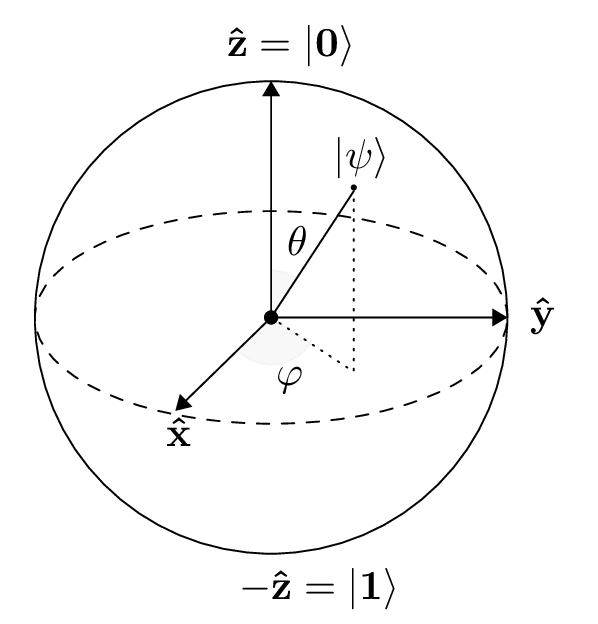
\includegraphics[width=0.5\linewidth]{img/img-ch2/bloch-sphere.png}
    \caption{The Bloch sphere representation of a qubit}
    \label{fig:bloch-sphere}
\end{figure}

\subsection{Quantum gates}
Postulates in \autoref{sec: measurements} and \autoref{sec: time evolution} highlighted the evolution of quantum states as well as their measurement. In quantum computing, time evolution operators are performed by quantum logic gates and measurements are done with respect to the computational basis. Next we will look at quantum gates. 

One-qubit quantum gates are formally described by $2 \times 2$ unitary transformations. 

\textbf{NOT gate}

The NOT gate, so-called X gate , is the quantum equivalent of the classical NOT gate. 
It is represented by the matrix
$$ X = \begin{bmatrix}
        0&1\\
        1&0\\
        \end{bmatrix} $$
It acts as:
\begin{align}
    \ket{0} &\longmapsto \ket{1} \\
    \ket{1} &\longmapsto \ket{0}
\end{align}
In other words, applied to a generic single-qubit state, the X gate swaps the amplitudes of the $\ket{0}$ and $\ket{1}$ components. 

Indeed, this gate corresponds to the Pauli X matrix. Coming back to the Bloch sphere, the X gate acts like a rotation of $\pi$ radians around the X axis of the Bloch sphere. We can generalize this behavior to obtain rotations of any angle around any axis of the Bloch sphere.

For the X axis we may define 
$$R_{X}(\theta)=e^{-i\frac{\theta}{2}X} = \begin{bmatrix}
        \cos \frac{\theta}{2}& -i \sin \frac{\theta}{2}\\
        -i \sin \frac{\theta}{2}& \cos \frac{\theta}{2}\\
        \end{bmatrix}$$
Analogously, for Y and Z axis:
\begin{align}
    R_{Y}(\theta)&=e^{-i\frac{\theta}{2}Y} = \begin{bmatrix}
        \cos \frac{\theta}{2}& - \sin \frac{\theta}{2}\\
        \sin \frac{\theta}{2}& \cos \frac{\theta}{2}\\
        \end{bmatrix}\\
    R_{Z}(\theta)&=e^{-i\frac{\theta}{2}Z} = \begin{bmatrix}
        e^{-i \frac{\theta}{2}}& 0\\
        0& e^{i \frac{\theta}{2}}\\
        \end{bmatrix}   
\end{align}

When $\theta=\pi$ the resulting matrices are known as \textbf{Pauli matrices}. Each of them define a quantum gate known as 
\begin{align}
    Y = R_{Y}(\pi)= \begin{bmatrix}
        0&-i\\
        i&0\\
        \end{bmatrix} \\
    Z = R_{Z}(\pi) = \begin{bmatrix}
        1&0\\
        0&-1\\
        \end{bmatrix} 
\end{align}

Another known gate coming from rotations of the Bloch sphere is the S gate which results from a $\frac{\theta}{2}$ rotation around the Z axis, known as \textbf{phase gate}:
$$ S = R_{Z}(\frac{\pi}{2})= \begin{bmatrix}
        1&0\\
        0&i\\
        \end{bmatrix} $$

\textbf{Hadamard gate}

Another remarkable gate is the Hadamard gate, denoted by H (which is not to be confused with the Hamiltonian also denoted by H). It is represented by the matrix
\begin{equation}
    H = \frac{1}{\sqrt{2}}\begin{bmatrix}
        1&1\\
        1&-1\\
        \end{bmatrix} 
\end{equation}

The Hadamard gate effect on the basis states $\ket{0}$ and $\ket{1}$ is 
\begin{align}
    \ket{0} &\longmapsto \frac{1}{\sqrt{2}}(\ket{0} + \ket{1}) \\
    \ket{1} &\longmapsto \frac{1}{\sqrt{2}}(\ket{0} - \ket{1})
\end{align}

Additionally, it is useful to keep in mind that
$$H = \frac{X+Z}{\sqrt{2}}$$

The role of the H gate is to create superposition of qubits.

For composite systems, we can guess that the tensor product will have a great importance again. The simplest way to build quantum gates on composite systems are tensor products of $2 \times 2$ unitary operators. In the case of two-qubit systems, the corresponding gates are $4 \times 4$ unitary operators constructed from the tensor product of two one-qubit quntum gates. Let $U_1$ and $U_2$ be one-qubit gates, the matrix of the gate $U_1 \otimes U_2$ is given by the tensor product of the matrices associated to $U_1$ and $U_2$:

\begin{align}
    U_1 \otimes U_2&=\begin{bmatrix}
        a_{11}&a_{12}\\
        a_{21}&a_{22}\\
        \end{bmatrix} 
    \otimes \begin{bmatrix}
        b_{11}&b_{12}\\
        b_{21}&b_{22}\\
        \end{bmatrix} 
    = \begin{bmatrix}
        a_{11} \begin{bmatrix}
        b_{11}&b_{12}\\
        b_{21}&b_{22}\\
        \end{bmatrix} &a_{12} \begin{bmatrix}
        b_{11}&b_{12}\\
        b_{21}&b_{22}\\
        \end{bmatrix} \\
        a_{21} \begin{bmatrix}
        b_{11}&b_{12}\\
        b_{21}&b_{22}\\
        \end{bmatrix} &a_{22} \begin{bmatrix}
        b_{11}&b_{12}\\
        b_{21}&b_{22}\\
        \end{bmatrix} \\
        \end{bmatrix} \\
    &= \begin{bmatrix}
        a_{11}b_{11}&a_{11}b_{12} &a_{12}b_{11}&a_{12}b_{12}\\
        a_{11}b_{21}&a_{11}b_{22}& a_{12}b_{21}&a_{12}b_{22}\\
        a_{21}b_{11}&a_{21}b_{12}& a_{22}b_{11}&a_{22}b_{12}\\
        a_{21}b_{21}&a_{21}b_{22}& a_{22}b_{21}&a_{22}b_{22}\\
        \end{bmatrix} 
\end{align}

By taking tensor products of one-qubit gates, we can only obtain operations that act on each qubit individually, but there are many unitary matrices that cannot be written as the tensor product of other matrices. A remarkable one is the controlled-NOT gate.

\vspace{5pt}
\textbf{CNOT gate}

The CNOT gate, known as controlled NOT gate is given by the unitary matrix
\begin{equation}
    CNOT = \begin{bmatrix}
        1&0&0&0\\
        0&1&0&0\\
        0&0&0&1\\
        0&0&1&0\\
    \end{bmatrix}
\end{equation}

It takes two input qubits, known as the control qubit and the target qubit. The state of the target qubit is changed, based  on the value of the control qubit. This is the principle of controlled gates. In particular, the CNOT gate, performs the NOT operation when the  control qubit is in state $\ket{1}$, otherwise, it remains unchanged. 

Next we will show how this gate acts on the elements of the two-qubit computational basis 

\begin{equation}
    CNOT \ket{00} = \ket{00},\quad  CNOT \ket{01} = \ket{01}, \quad CNOT \ket{10} = \ket{11}, \quad  CNOT \ket{11} = \ket{10}
\end{equation}

More generally, given an arbitrary qubit unitary operation denoted by $U$. A controlled $U$ operation is a two qubit transformation, again with a control and a target qubit. If the control qubit is set, then $U$ is applied to the target qubit, otherwise the target qubit is left alone.

The previously presented quantum gates are summarised at \autoref{tab: quantum gates}.

\begin{table}
    \centering
    \begin{tabular}{ccc}
    \toprule
        Gate     & Circuit representation    & Matrix \\
        \hline 
        \addlinespace
        X-Pauli (NOT) & \begin{quantikz} & \gate{X} & \qw\\ \end{quantikz} \egroup {& $\begin{bmatrix} 0&1\\1&0  \end{bmatrix}$\\
        Y-Pauli & \begin{quantikz} & \gate{Y} & \qw\\ \end{quantikz} \egroup {& $\begin{bmatrix} 0&-i\\i&0  \end{bmatrix}$\\
        Z-Pauli & \begin{quantikz} & \gate{Z} & \qw\\ \end{quantikz} \egroup {& $\begin{bmatrix} 1&0\\0&-1  \end{bmatrix}$\\
        Phase & \begin{quantikz} & \gate{S} & \qw\\ \end{quantikz} \egroup {& $\begin{bmatrix} 1&0\\0&i  \end{bmatrix}$\\
        Hadamard & \begin{quantikz} & \gate{H} & \qw\\ \end{quantikz} \egroup {& $\frac{1}{\sqrt{2}}\begin{bmatrix} 1&1\\1&-1  \end{bmatrix}$\\
        CNOT & \begin{quantikz} \lstick{} & \ctrl{1} & \qw\\ \lstick{} & \targ{} & \qw\\ \end{quantikz} \egroup {& $\begin{bmatrix} 1&0&0&0\\ 0&1&0&0\\ 0&0&0&1\\ 0&0&1&0\\\end{bmatrix}$\\
    \end{tabular}
    \caption{Summary table of useful quantum logic gates and their representations}
    \label{tab: quantum gates}
\end{table}

Departing from this overview of quantum gates we have the basis to build more complex gates and circuits.

\section{Open quantum systems}
As we have briefly mentioned in previous sections, the most widely treated and studied quantum systems are those called closed systems, which are the ones that only interact with themselves, isolated from the rest of the universe. By definition, it is a system which does not interchange information with another system. All the previous description of quantum mechanics was built in the realm of closed quantum systems. However, beyond theoretical level, closed quantum systems are not that relevant because no system can be completely isolated from its environment in the real world. Indeed, for this to happen, it would be needed a sort of ``infinite barrier'' around the system in question that cannot be recreated in an experimental environment. Therefore, since no quantum system is completely isolated from its surroundings, it is important to develop a theoretical framework for treating these interactions in order to obtain an accurate understanding of quantum systems. We have decided to introduce the notion of open quantum systems, a quantum mechanical system that interacts with an external quantum system, which is known as the environment or bath. We will analyze its evolution considering that it is not isolated from the rest of the universe and the mutual actions between the system and the environment. 


\begin{definicion}[Open quantum system]
    An open quantum system is a quantum mechanical system $S$, which is associated to a Hilbert space $\mathbb{H}_S$, that is interacting with another quantum system $E$: the environment, which is associated to a Hilbert space $\mathbb{H}_E$. Let's assume that $\dim (\mathbb{H}_S)=n$ and $\dim(\mathbb{H}_E)=n$. \\Therefore, $S$ is a subsystem of the total system $(S+E)$, whose corresponding Hilbert space is the tensor product $\mathbb{H}_T=\mathbb{H}_S \otimes \mathbb{H}_E$, that is $nm$-dimensional.
\end{definicion}

Traditionally, the time evolution of quantum systems has been described through a unitary transformation that connects the states of the system at two points in time. However, this description becomes excessively restrictive when attempting to analyze the time evolution of an open quantum system. To understand how the open quantum system that we have just defined evolves in time we will denote $H_s$ the open quantum system Hamiltonian, $H_e$ the environment Hamiltonian and $H_{se}$ the system-environment interaction Hamiltonian. Assuming that the entire open quantum system is a large closed system, its time evolution is governed by a unitary transformation generated by a global Hamiltonian given by
$$H = H_s \otimes I_e + I_s \otimes H_e + \alpha H_{se}$$
where $I_s$ and $I_e$ are the identity operators of the system and environment Hilbert spaces respectively, $\alpha$ is a coupling constant that depends on the interaction between the system and the environment. 

Since the system $S+E$ evolves according to a unitary time evolution operator $U(t,t_0)$, the density operator of the composite system at an initial time $t_0$ is described by a density matrix $\rho(t_0)$. The density operator at a time $t$ is given by $\rho(t)=U(t,t_0)\rho(t_0) U^{\dag}(t,t_0)$. The quantum states of the subsystems $S$ and $E$ at time $t$ are represented by their respective reduced density operators denoted by $\rho_S(t)$ and $\rho_E(t)$. These operators contain all the relevant statistical information for potential measurements performed on each subsystem. To obtain $\rho_S(t)$ and $\rho_E(t)$, it is needed to calculate the partial trace of $\rho(t)$ with respect to the degrees of freedom of $E$ and $S$, respectively.
\begin{align}
    \rho_S(t) &= \mathrm{Tr}_E(\rho(t)) \\
    \rho_E(t) &= \mathrm{Tr}_S(\rho(t))
\end{align}

\begin{definicion}[Partial trace]
    Let $X,Y$ be finite vector spaces of dimension $n$ and $m$ respectively. The partial trace over $Y$ is a linear operator defined as $\mathrm{Tr}_Y: \mathcal{L}(X \otimes Y) \longrightarrow \mathcal{X} $ such that
    $$\mathrm{Tr}_Y(T \otimes U) = \mathrm{Tr}(U) T \quad \forall T \in \mathcal{L}(X), \, \forall U \in \mathcal{L}(Y) $$

    Analogously, the partial trace over $X$ is $\mathrm{Tr}_X: \mathcal{L}(X \otimes Y) \longrightarrow \mathcal{Y} $ such that
    $$\mathrm{Tr}_X(T \otimes U) = \mathrm{Tr}(T) U \quad \forall T \in \mathcal{L}(X), \, \forall U \in \mathcal{L}(Y) $$
\end{definicion}

As the density operator of the environment is positive and normalized, it has a spectral decomposition in an orthonormal basis with non negative eigenvalues. Hence, 
$$\rho_E(t)=\sum_{v}\lambda_v \ket{v}\bra{v}$$
where $\lambda_v$ are the eigenvalues and $\left\lbrace \ket{v}\right \rbrace $ are the corresponding orthonormal eigenvectors.

We can express the reduced density operator of $S$ performing the partial trace in the orthonormal basis of the environment eigenstates:
\begin{align}
    \rho_s(t)&=\mathrm{Tr}_E\left[(U(t,t_0) \rho(t_0) U^{\dag}(t,t_0)\right] \\
    &= \sum_{\mu} \braket{\mu | U(t,t_0) \rho(t_0) U^{\dag}(t,t_0) | \mu}
\end{align}

We will assume, as is customary, that at the initial time the density operator of the closed system $S+E$ is separable, that is $\rho(t_0) = \rho_S(t_0)\otimes \rho_E(t_0)$ and that the reduced density operator $\rho_E(t_0)$ is equal to a certain fixed value $\rho_{E,0}$ regardless of the value of $t_0$. Then, the initial state of the total system at $t_0$ would be $\rho(t_0) = \rho_S(t_0)\otimes \rho_{E,0}$. It follows that
\begin{align}
    \rho_S(t)&=\mathrm{Tr}_E\left[ U(t,t_0) \rho_S(t_0) \otimes \rho_{E,0} U^{\dag}(t,t_0) \right] \\
    &= \sum_{\mu v} K_{\mu v}(t, t_0) \rho_S(t_0) K_{\mu v}^{\dag}(t, t_0) 
\end{align}
where $K_{\mu v}(t,t_0)$ are operators acting on the Hilbert space of $S$, known as Kraus operators. They are given by 
$$K_{\mu v}(t,t_0) = \sqrt{\lambda_v}\braket{\mu | U(t,t_0) | v}$$

The equation defining the system in terms of Kraus operators is called the Kraus Operator Sum representation. 

Just as the Schrödinger equation describes how pure states evolve in time, the equation governing the temporal evolution of the density operator of a closed quantum system is the Liouville-von Neumann equation
\begin{equation}
    \frac{d \rho(t)}{d t} = -\frac{i}{\hbar}\left[ H(t), \rho(t)\right]
\end{equation}
where $H(t)$ represents the Hamiltonian of the system, the square brackets denote the commutator of the operators enclosed within and $\hbar$ is Planck's constant.

By the Taylor expansion around $t=0$ we have:
$$\rho(dt)=\rho(0) + \frac{d \rho (t)}{dt}|_{0} + O(dt^2)$$
Using the Kraus Operator Sum representation,
$$\rho(dt)=\sum_{\alpha} K_{\alpha}(dt) \rho(0) K_{\alpha}^{\dag}(dt)$$
where we have collected the $\mu v$ indices into a single index $\alpha$.

It can be shown (\cite{lidar2019lecture}) that the reduced density operator of $S$ fulfills the evolution equation 
\begin{equation}
    \frac{d \rho_S(t)}{d t}|_{0} = -\frac{i}{\hbar}\left[ H_S, \rho_S(0)\right] + \sum_{j=1}^{n^2-1}\gamma_j \left[ L_j\rho_S(0) L_j^{\dag} - \frac{1}{2}(L_j^{\dag}L_j, \rho_S(0) )\right]
\end{equation}
This result is valid as a short time expansion near $t=0$. Making the assumption that the previous equation is valid for all times $t>0$, which is essentially the Markovian limit, that states that there is no memory in the evolution, as manifested by the fact that the evolution resets every $dt$. This takes us to

\begin{equation}
    \frac{d \rho_S(t)}{d t} = -\frac{i}{\hbar}\left[ H_S(t), \rho_S(t)\right] + \sum_{j=1}^{n^2-1}\gamma_j(t) \left[ L_j(t) \rho_S(t) L_j^{\dag}(t) - \frac{1}{2}(L_j^{\dag}(t)L_j(t), \rho_S(t) )\right] = \mathcal{L}\rho
\end{equation}
 
where $H_S(t)$ is an operator playing the role of the Hamiltonian for $S$ but which also contain information about the environment $E$, $n$ is the dimension of the Hilbert space of $S$, $\left\lbrace \gamma_j(t) \right\rbrace_{j=1}^{n^2-1}$ is a set of nonnegative functions with dimensions of frequency, $\left\lbrace L_j(t) \right\rbrace_{j=1}^{n^2-1}$ is a set of dimensionless operators known as Lindblad operators or quantum jump operators, and the braces denote the anticonmmutator of the operators enclosed within. This equation is known as \textbf{Gorini-Kossakowski-Sudarshan-Lindblad} (GKSL) equation or simply as the \textbf{Lindblad master equation}. The first term on the right-hand of the equation represents the unitary evolution of the system, whereas the second term describes the dissipative aspect of the dynamics. In the typical case where the time evolution operator $U(t,t_0)$ is invariant under temporal translations, that is $U(t+ \tau, t_0 + \tau) =U(t,t_0), \, \forall t,t_0,\tau \in\mathbb{R}$, then $H(t)$, $L_j(t)$ and $\gamma_j(t)$ become constants, resulting in a time-independent Lindblad master equation.

The generator of the evolution, $\mathcal{L}$ is called the Lindblandian. The form of the dissipative part of the Lindblandian, is 
$$\mathcal{L}_D[\cdot] = \sum_{j=1}^{n^2-1}\gamma_j \left[ L_j\rho_S(0) L_j^{\dag} - \frac{1}{2}(L_j^{\dag}L_j, \rho_S(0) )\right], \quad \gamma_j >0$$

We can now define the decoherence phenomena. Decoherence is what happens when $\mathcal{L}_D \neq 0$. This means that the evolution of the density matrix is governed not only by the Liouville-von Neumann component $\frac{-i}{\hbar}[H, \cdot]$ responsible for the unitary evolution, but also by the dissipator, which gives rise to non-unitary evolution. 

The formal solution of the Lindblad equation 
$\frac{d \rho_S(t)}{d t} = \mathcal{L}\rho_S$ is $$\rho_S(t) = e^{\mathcal{L}t} \rho_S(0) \equiv \Lambda(t) \rho_S(0) $$

For a certain $t$, the application $\Lambda(t)$ is called a dynamic application. If we consider the family of maps over time generated by the GKSL equation we obtain a one-parameter family $\left\lbrace \Lambda(t) : \, t \geq 0 \right \rbrace$ of dynamic applications that satisfy the following properties:
\begin{enumerate}
    \item Identity operator: $\Lambda(0)=\mathbb{1}$
    \item Closed under multiplication: since we are assuming a Markovian behaviour, it follows the Markov property,
    $$\Lambda(t_1)\Lambda(t_2) = \Lambda(t_1+t_2), \quad t_1, t_2 \geq 0$$
    which is also the property of the semigroup.
    \item Associative: $(\Lambda(t_1)\Lambda(t_2))\Lambda(t_3) = \Lambda(t_1)(\Lambda(t_2)\Lambda(t_3))$
\end{enumerate}

Therefore, the family of one-parameter dynamic applications generated by the GKSL equation form a \textbf{quantum dynamical semigroup}. For providing the definition of this structure, first we need to introduce the following notions.

Let $X$ be a Banach space and let $f \in X^*$. We denote $\varphi_f: X \longrightarrow \mathbb{R}$ the linear functional $\varphi_f(x)=\braket{f,x}$. As $f$ runs through $X^*$ we obtain a collection $\left \lbrace \varphi \right\rbrace_{f \in X^*}$ of maps from $X$ into $\mathbb{R}$. We define a new topology on the set $X$:

\begin{definicion}[Weak topology]
    The weak topology $\sigma(X, X^*)$ on $X$ is the coarsest topology associated to the collection $\left \lbrace \varphi_f \right\rbrace_{f \in X^*}$
\end{definicion}

We are now going to define a topology on $X^*$ called the \textbf{weak$^*$ topology} and denoted by $\sigma(X^*,X)$. For every $x\in X$ consider the linear functional $\varphi_x: X^* \longrightarrow \mathbb{R}$ defined by $f \longmapsto \varphi_x(f)=\braket{f,x}$. As $x$ runs through $X$ we obtain a collection $\left\lbrace \varphi _x \right\rbrace_{x\in X}$ of maps from $X^*$ into $\mathbb{R}$.

\begin{definicion}[Weak$^*$ topology]
    The weak$^*$ topology $\sigma(X^*,X)$ is the coarsest topology on $X^*$ associated to the collection $\left\lbrace \varphi _x \right\rbrace_{x\in X}$
\end{definicion}

Next, we will characterise the notion of convergence in these topologies.
\begin{definicion}
    \begin{itemize}
        \item A sequence $\left\lbrace x_n \right \rbrace$ in $X$ converges to $x$ in the weak topology $\sigma(X,X^*)$,
        $$x_n \rightharpoonup x $$
        if and only if $$\braket{f,x_n} \longrightarrow \braket{f,x}\, \forall f \in X^*$$

        \item A sequence $\left\lbrace f_n \right\rbrace$ in $X^*$ converges to $f$ in the weak$^*$ topology $\sigma(X^*,X)$, 
        $$f_n \stackrel{*}{\rightharpoonup} f $$
        if and only if 
        $$\braket{f_n,x}\longrightarrow \braket{f,x},\, \forall x \in X$$
    \end{itemize}
\end{definicion}

It is worth pointing out that if $f_n \stackrel{*}{\rightharpoonup} f $ in $\sigma(X^*,X)$ and $x_n \rightharpoonup x$ in $\sigma(X,X^*)$, in general, one cannot conclude that $\braket{f_n,x_n} \longrightarrow \braket{f,x}$. 

Now, we will briefly go through some concepts of the theory of Banach algebras, a large are in functional analysis. We will assume that the underlying field of scalars $\mathbb{K}$ is the field of complex numbers $\mathbb{C}$. An algebra over $\mathbb{C}$ is a vector space $\mathcal{A}$ over $\mathbb{C}$ that also has a multiplication defined on it that makes $\mathcal{A}$ into a ring such that if $\alpha \in \mathbb{C}$ and $a,b \in \mathcal{A}$, $\alpha(ab)=(\alpha a)b = a(\alpha b)$

\begin{definicion}[Banach algebra]
    A Banach algebra is an algebra $\mathcal{A}$ over $\mathbb{C}$ that has a norm $||\cdot||$ relative to which $\mathcal{A}$ is a Banach space and such that for all $a,b \in \mathcal{A}$,
    $$||ab|| \leq ||a||\,||b||$$
\end{definicion}

A $C^*$-algebra is a particular type of Banach algebra that is intimately connected with the theory of operators on a Hilbert space.

If $\mathcal{A}$ is a Banach algebra, an \textbf{involution} is a map 
\begin{align}
    \mathcal{A} &\longrightarrow \mathcal{A} \\
    a &\longmapsto a^*
\end{align}
such that the following properties hold for $a,b \in \mathcal{A},\, \alpha \in \mathbb{C}$:
\begin{enumerate}
    \item $(a^*)^*=a$
    \item $(ab)^* = b^*a^*$
    \item $(\alpha a +b)^* = \bar{\alpha}a^* +b^*$
\end{enumerate}

\begin{definicion}[$C^*$-algebra]
    A $C^*$-algebra is a Banach algebra $\mathcal{A}$ with an involution such that for every $a$ in $\mathcal{A}$,
    $$ ||a^*a||=||a||^2$$
\end{definicion}

\begin{definicion}[Von-Neumann algebra]
    A Von-Neumann algebra $\mathcal{A}$ is a $C^*$-algebra of the bounded operators $\mathcal{B}(\mathbb{H})$ in a Hilbert space that is closed under the weak$^*$ topology and contains the identity $I \in \mathcal{B}(\mathbb{H})$
\end{definicion}
 
Lastly, we can define the concept of quantum dynamical semigroups.
\begin{definicion}[Dynamic semigroup]
    Let $\mathcal{A}$ be a von-Neumann algebra. A dynamic semigroup is defined as a one-parameter family of applications $\Phi_t: \mathcal{A} \longrightarrow \mathcal{A}$ with the following properties:
    \begin{enumerate}
        \item $\Phi_t$ is positive for all $t\geq 0$
        \item $\Phi_t(I)=I$
        \item $\Phi_s \cdot \Phi_t = \Phi_{s+t}$
        \item $\Phi_t(X) \stackrel{*}{\rightharpoonup} X$ when $t \longrightarrow 0$
        \item $\Phi_t$ is weakly$^*$ continuous operator in $\mathcal{A}$
    \end{enumerate}
\end{definicion}

\section{Closing remarks}
The revolution in the world of physics in the 1920s led to the creation of quantum mechanics, an indispensable part of science ever since. Quantum computing emerges from this field, as proposed by Richard Feynman, in order to understand and simulate it.

Another major triumph of the 20th century was computer science. Within a century, there were proposals for the Turing machine, the construction of the first computers, and hardware development. In 1965, Gordon Moore declared that computational power would double at a constant cost every two years, meaning that the number of transistors in a microprocessor would double every two years. However, there is a limit to this due to quantum effects interfering with the operation of increasingly smaller electronic components. To overcome this barrier, one possible solution is to shift the computing paradigm: quantum computing.

In essence, quantum computing is the union of both branches, but after its invention and theoretical formulation: What are its possibilities? Quantum computing surpasses classical computing for some specialized tasks. The potential applications of quantum computing are still to be determined as it does not provide efficient solutions to all problems. However, this does not mean that quantum computing is an illusion or mere theory. Quantum algorithms have been developed, such as the famous Grover's Algorithm (for searching an unstructured search space) and Shor's Algorithm (for factorizing a number). The field of quantum information theory has been created, encompassing quantum computing, cryptography, and quantum communication. Furthermore, progress has been made in the theory of quantum error correction to protect data integrity.

On the other hand, companies are in a race to build quantum computers and have made many tools available to researchers and developers to program quantum algorithms and run them on their computers, such as IBM Quantum Composer and Quantum Lab, IBM's Qiskit, Google Quantum AI's Cirq, PennyLane, D-Wave's Leap, and many more.

Quantum computing will coexist with classical computing; it is not a paradigm that will replace the other, as both have their strengths. It is a burgeoning new field with challenges and questions to investigate, engaging physicists, engineers, and mathematicians in research groups and companies today.

\endinput
%--------------------------------------------------------------------
% FIN DEL CAPÍTULO. 
%--------------------------------------------------------------------
